% !TeX root = ../main.tex

\chapter{组装与调试}
\label{cha:chapter03}
本项目选择把跳跃和滑翔分开作为两个独立的过程来分析与控制,用一个无刷电机驱动跳跃部分,用一个舵机控制机翼的开合。
\section{理论计算}
\label{sec:calculations}
取$g=9.8m/s^2$,预计机器人重量$m=200g$,跳跃高度$h=1m$,起跳电机做功时间$t=0.1s$,则机器人所需最小动能:
\begin{equation}
\label{equ:chap2:W_calc}
W_k=mgh
\end{equation}
二级齿轮减速器机械效率估计为$\eta=80\%$,则所需电机输出最小平均功率:
\begin{equation}
  \label{equ:chap2:P_calc}
  \bar{P}_{min}=\frac{W_k}{t·\eta}
  \end{equation}
解得:$$\bar{P}_{min}=24.5(W)$$
二级齿轮减速器减速比大约在10\sim30:1,设计中一次起跳输出级齿轮大约需要转半圈,取减速比20:1,则所需无刷电机转速:
$$\omega_{min}=0.5\times10\div t\times60=6000(rpm)$$
使用2S锂离子电池,额定电压$V=7.4V$,则所需最小电机KV值:
$$KV_{min}=\omega_{min}\div V=810(rpm/V)$$
一般来讲KV值越小无刷电机转矩越大,根据计算及机械需求考虑,选择了最大功率$P_{max}=168W$的朗宇X2305航模无刷电机,KV值$KV=1450$。\\
机器人起跳最小速度:
\begin{equation}
  \label{equ:chap2:v_calc}
  v=\sqrt{2gh}
  \end{equation}
根据动量定理:
\begin{equation}
  \label{equ:chap2:motion_principle}
  \bar{F}·t=m·v
  \end{equation}
解得所需平均力:$$\bar{F}=8.854(N)$$
航模用无刷电机的力矩数据不好获得,我们通过相同工作条件下的带螺旋桨升力进行估算,实际输出力只会更大。电机参数显示6000rpm时的升力等效质量约为$m_f=200\sim300g$,即经减速器输出的力为:$$F_min=m_{f,min}·g·20=39.2(N)>\bar{F}$$
此处还未考虑腿部连杆结构带来的机械增益,而其均值应>1,因此理论上输出力是足够支持跳跃的。
\section{元件选型}
\label{sec:components}
根据上述计算过程与现实考量,选择元件如表\ref{tab:bom}所示。
\begin{table}[htb]
  \centering
  \begin{minipage}[t]{0.8\linewidth}
  \caption{BOM表}
  \label{tab:bom}
    \begin{tabularx}{\linewidth}{lX}
      \toprule[1.5pt]
      {\heiti 元件名} & {\heiti 描述} \\\midrule[1pt]
      朗宇X2305无刷电机 & 外转子无刷电机,KV值1450 \\
      NanoPi Duo2 开发板 & 全志H3主控,运行Ubuntu 18.04\\
      FOC电机控制板 &  基于STSPINF0A方案的BLDC矢量控制 \\
      EMAX 2S航模锂电池 & 容量300mAh,质量为15g\\
      DS-S002M 4.3g数字舵机 & 用于控制机翼开合\\
      OV5640摄像头 & 500W像素,1080p@30fps,720p@60fps\\
      \bottomrule[1.5pt]
    \end{tabularx}
  \end{minipage}
\end{table}
\section{机械设计}
\label{sec:mechanical}
初步设计的机器人整体结构三维仿真图如下(螺丝等固定细节略去):
\begin{figure}[H]
  \centering
  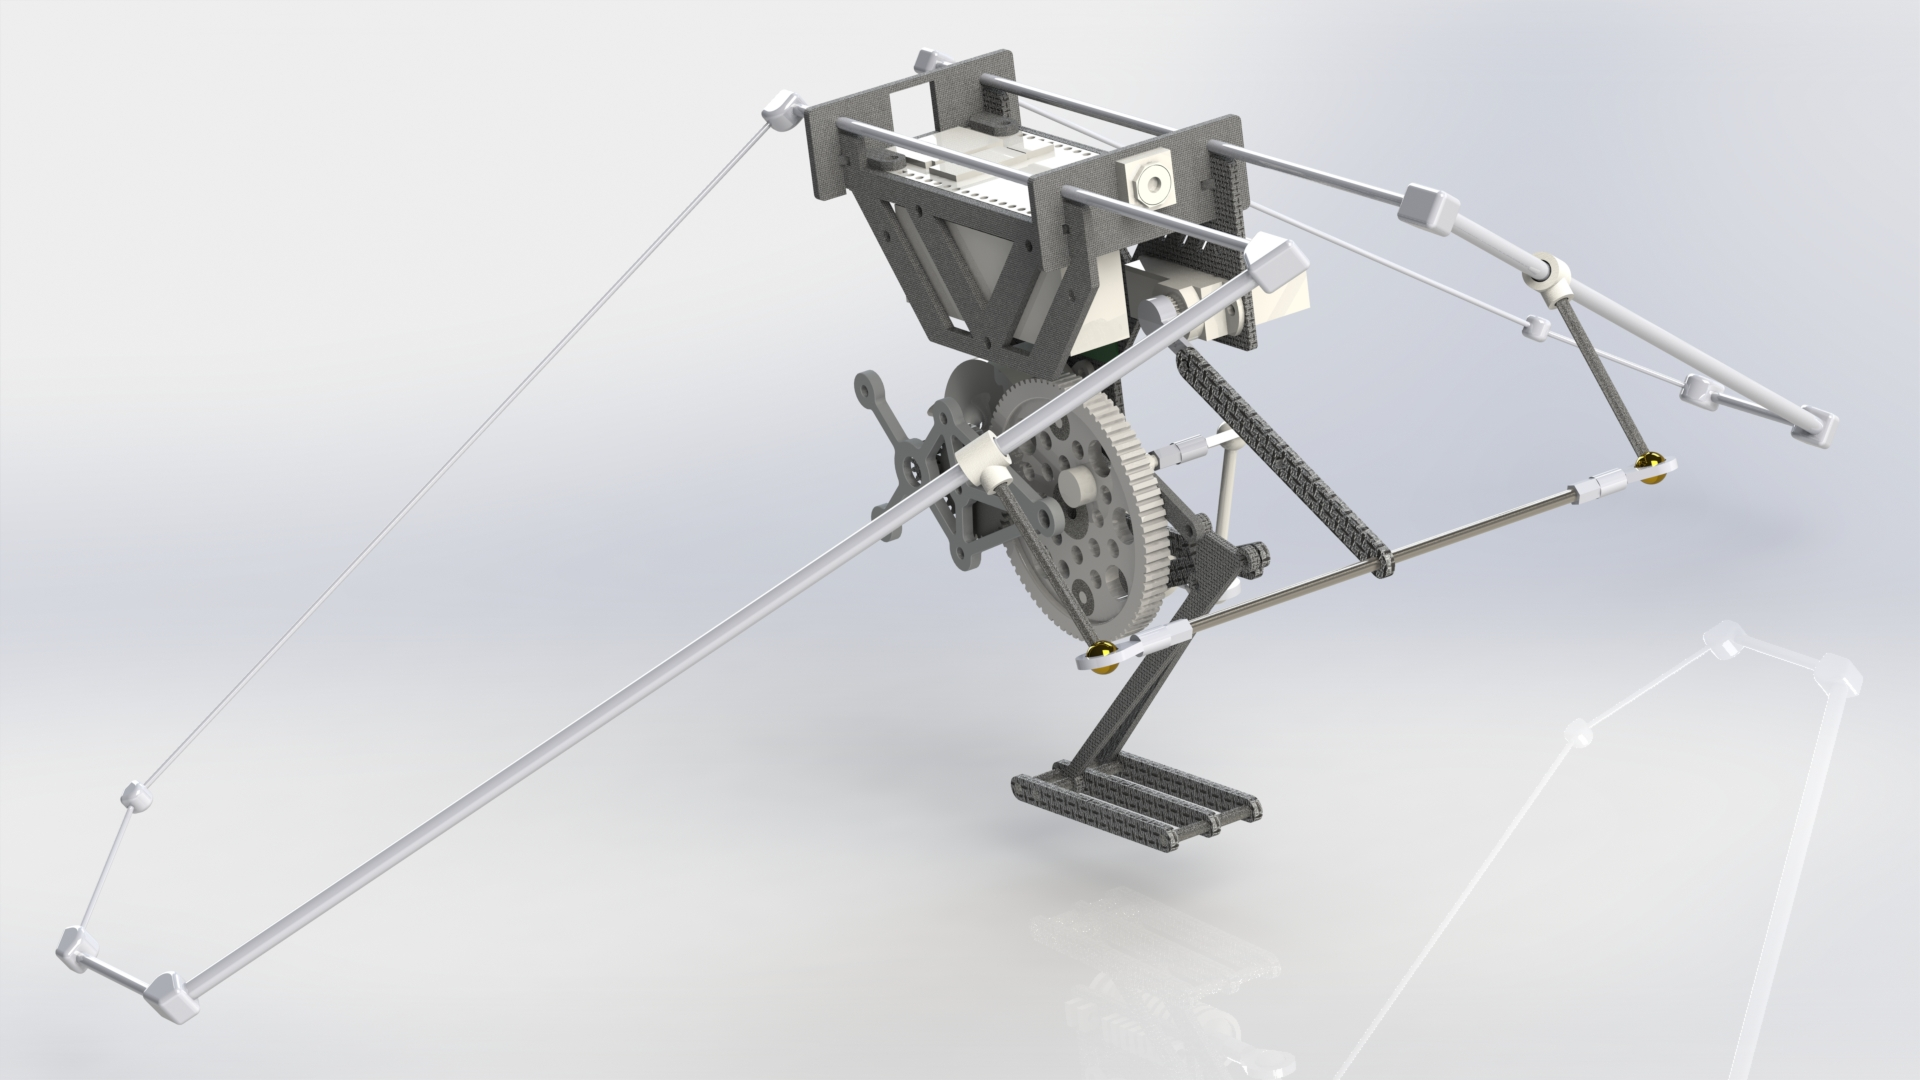
\includegraphics[height=8cm]{render2.jpg}
  \caption{整体结构渲染图}
  \label{fig:render_v1}
\end{figure}
\subsection{减速器设计}
设计目标为减速比20:1的两级齿轮减速器。考虑本项目实际尺寸,选用模数为0.5或0.6的齿轮较为合适。在市面上可直接买到的齿轮中,选择了0.5模数15齿的主轴齿轮,10/36齿的次级双层齿轮和80齿的末级齿轮。其中主轴齿轮材料为铜(粉末铸造),次级齿轮为铁基齿轮,而体积最大的末级齿轮采用了铝合金材质,兼顾了硬度与重量。

\begin{figure}[H]
  \centering
  \subcaptionbox{主轴齿轮\label{fig:cog1}}[4cm] 
    {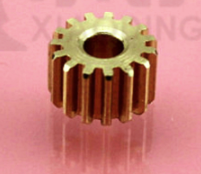
\includegraphics[height=3cm]{cog15.png}}
  \hspace{3em}
  \subcaptionbox{次级齿轮\label{fig:cog2}}[3cm]
      {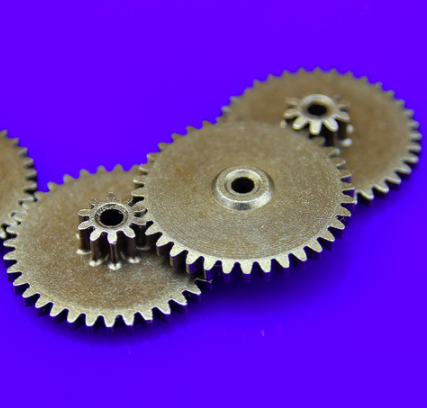
\includegraphics[height=3cm]{cog10_36.png}}
  \hspace{4em}
  \subcaptionbox{末级齿轮\label{fig:cog3}}
      {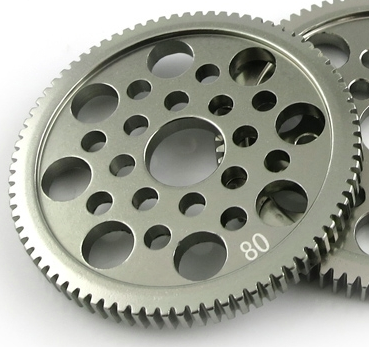
\includegraphics[height=3cm]{cog80.png}}
  \caption{齿轮的选择}
  \label{fig:cogs}

\end{figure}

据此我们设计出用于固定的减速器支架,选择铝合金材质CNC而成,保证连接强度的同时尽量减轻质量。设计图与实物图如图\ref{fig:retarder}所示,装配示意图如图\ref{fig:retarder_assembly}所示。
\begin{figure}[H]
  \centering
  \subcaptionbox{减速器模型\label{fig:retarder_model}}[7cm] 
    {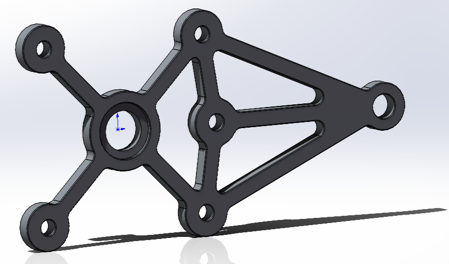
\includegraphics[height=4cm]{retarder_model.png}}
  \hspace{4em}
  \subcaptionbox{减速器实物\label{fig:retarder_real}}
      {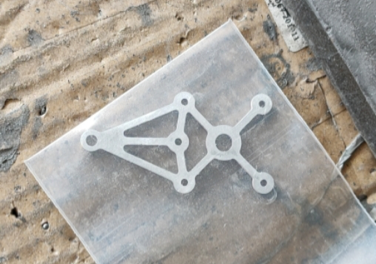
\includegraphics[height=4cm]{retarder_real.png}}
  \caption{减速器}
  \label{fig:retarder}
\end{figure}
\begin{figure}[H]
  \centering%
  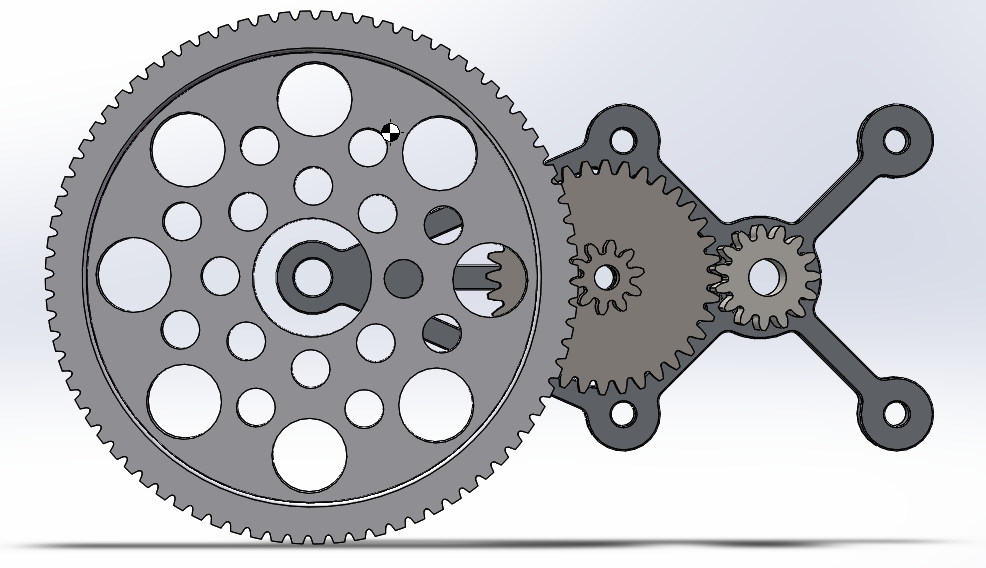
\includegraphics[height=8cm]{retarder_assembly.png}
  \caption{减速器装配图}
  \label{fig:retarder_assembly}
\end{figure}
\subsection{腿部设计}
参考Salto\cite{Salto}的腿部模型,此处实现了如图\ref{fig:2d_leg_fold}和图\ref{fig:2d_leg_stretch}所示的连杆结构。其中灰色圆为输出级齿轮,带动上部的曲柄-摇臂四连杆结构,同时四连杆摇臂为一凹四边形块,与机身相连的另一点在下部又组成了一个平行四边形四连杆,在输出级利用杠杆结构增大位移,实现触地端的较大速度,从而使身体跳起。虽然看上去略显复杂,但总体形态接近自然界大多数生物的腿部构造,这也从一个侧面反映了该结构的合理性。

\begin{figure}[H]
  \centering%
  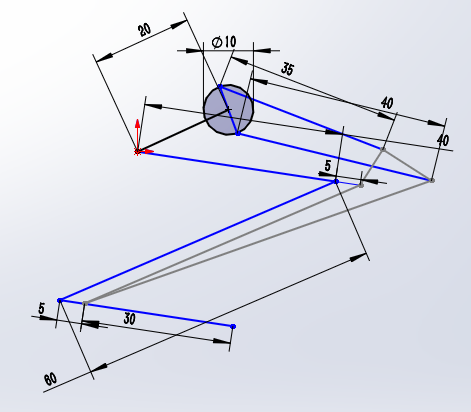
\includegraphics[height=6cm]{2d_leg_fold.png}
  \caption{起跳前准备姿势}
  \label{fig:2d_leg_fold}
\end{figure}
\begin{figure}[H]
  \centering%
  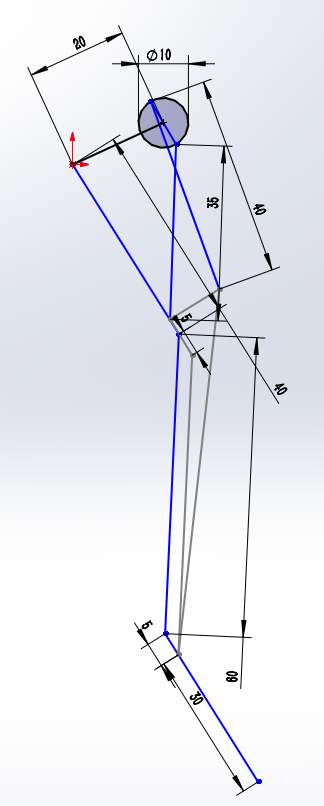
\includegraphics[height=11cm]{2d_leg_stretch.png}
  \caption{起跳后空中姿势}
  \label{fig:2d_leg_stretch}
\end{figure}

据此尺寸在SolidWorks中设计出三维模型,装配示意图如图\ref{fig:3d_leg}所示。
\begin{figure}[H]
  \centering%
  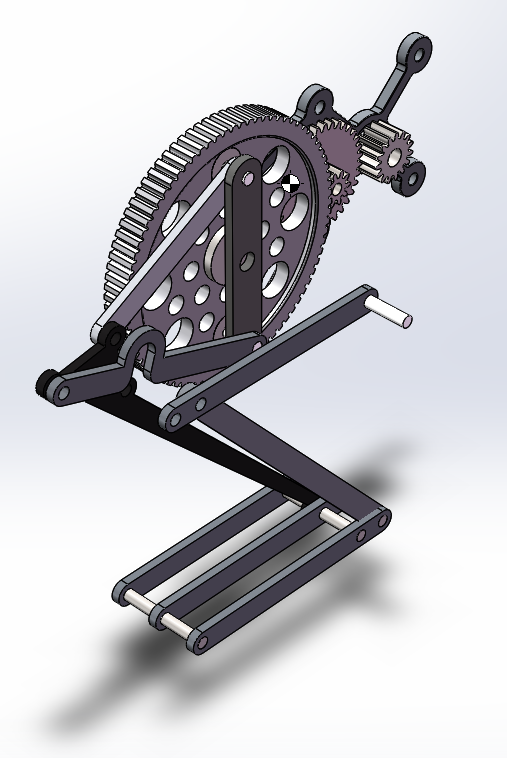
\includegraphics[height=8cm]{3d_leg.png}
  \caption{腿部装配图}
  \label{fig:3d_leg}
\end{figure}

\subsection{机翼设计}
\label{sec:wings}
采用蝴蝶式\cite{EPFL}折叠机翼设计,利用一个小舵机带动两片机翼的同步开合。为了降低机翼质量,采用碳纤维骨架与蒙皮的形式,骨架由碳纤维杆与3D打印的接头组成,翼面材料使用潍坊风筝布料,以保证强度与抗老化性。机翼部分
\begin{figure}[H]
  \centering%
  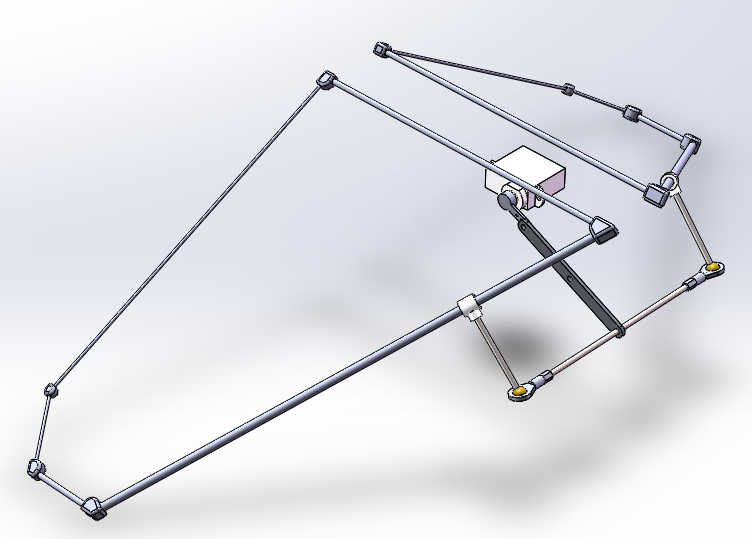
\includegraphics[height=8cm]{wings_mechanism.png}
  \caption{机翼原理图}
  \label{fig:wings_mechanism}
\end{figure}
